\subsection{Three shared memory implementations}

We have compared three different implementation for shared memory parallelisation: 
\begin{enumerate}
\item ``R-side parallelism'', a high level R multi-threading which uses
  \texttt{mclapply} from the R \texttt{parallel} package.
\item ``naive openMP'' which encloses the map step with \texttt{\#pragma
    omp parallel} and \texttt{\#pragma omp for}, and protects the
  global report object (reduction step) with \texttt{\#pragma omp
    critical}
\item ``improved openMP'', where the reduction step was refactored by
  first performing a thread-wise reduction in a thread-private report
  object and then finally reduced in the end report.
\end{enumerate}
\begin{figure}[!htbp] \centering
  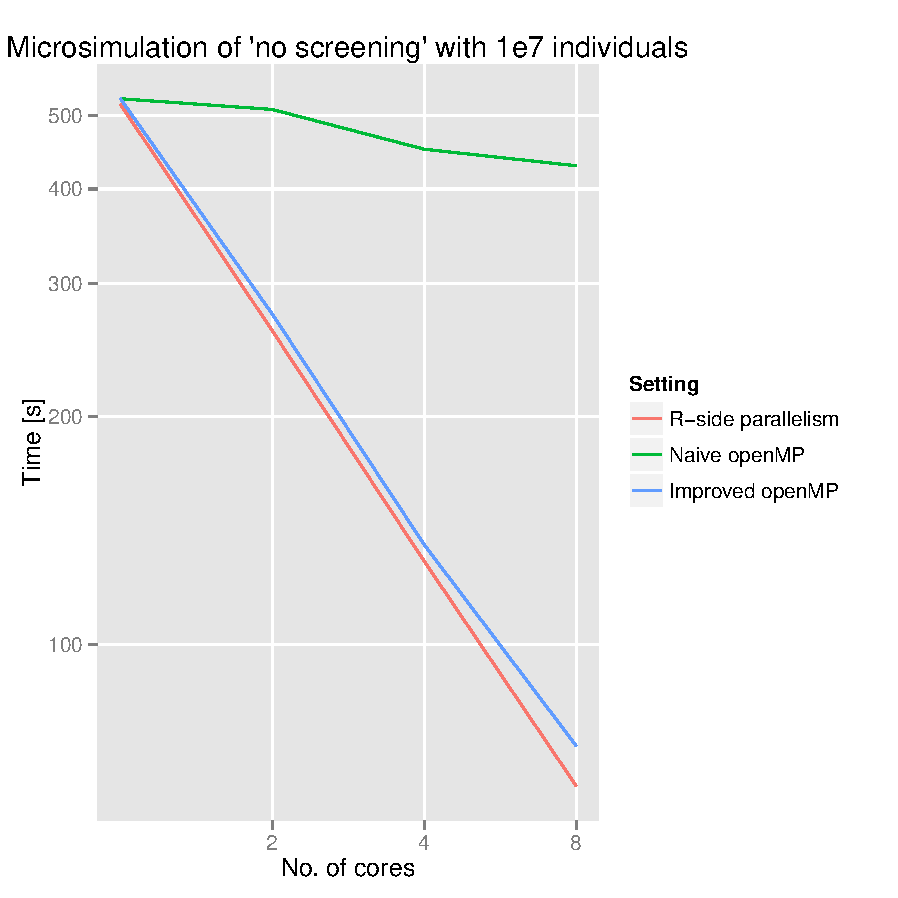
\includegraphics[height=0.5\textheight]{images/implementationProfiling.pdf}
  \caption{The execution times of the three different implementations
    described in the text. The difference between the ``naive openMP''
  and ``improved openMP'' is the local update to the report
  object.}
  \label{fig:implScaling}
\end{figure} 
Figure \ref{fig:implScaling} shows how the three
different implementations of parallelisation scales with additional
cores. The ``R-side parallelism'' and ``Improved openMP'' scales
well with comparable results. The ``Naive openMP'' implementation
with the ``EventReport'' mentioned in Figure \ref{fig:cppMot} within
\texttt{\#pragma omp critical} statements scales very poorly. 

Given the data, the automatic R-side parallelism should be
used. However, it does not scale beyond a single node, so if one wants
to run a significant larger population, then the combination \texttt{openMP
+ MPI} could be used.


%%% Local Variables: 
%%% mode: latex 
%%% TeX-master: "report" 
%%% End:
